\documentclass[tikz,border=2pt]{standalone}
\usepackage{amsmath}
\usepackage{pgfplots}
\pgfplotsset{compat=1.18}
\usetikzlibrary{arrows.meta}
\begin{document}
% X ~ Bernoulli(0.2), Y ~ Bernoulli(0.4): F_X = 0.8 and F_Y = 0.6 on [0,1), both 0 before 0 and 1 from 1 on,
% so F_X(t) >= F_Y(t) for every t, i.e. X <=_st Y (gap 0.2 = P(Y>t) - P(X>t) on [0,1)).
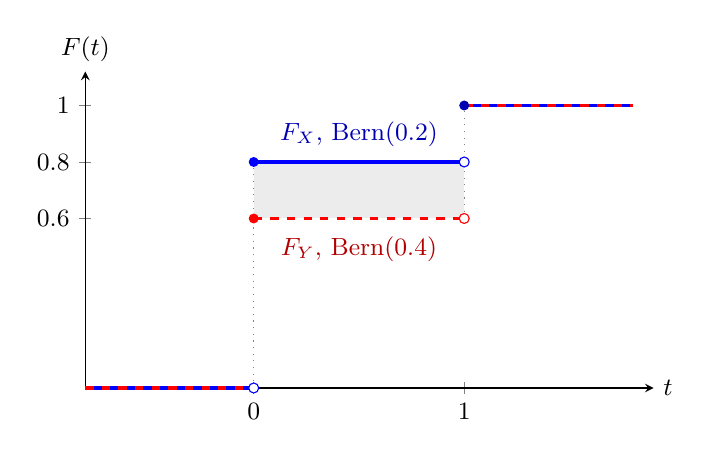
\begin{tikzpicture}[font=\small, >={Latex[length=2mm]}]
  \begin{axis}[
    axis lines=left, xmin=-0.8, xmax=1.9, ymin=0, ymax=1.12,
    xtick={0,1}, ytick={0.6,0.8,1},
    xlabel={$t$}, ylabel={$F(t)$},
    xlabel style={at={(axis description cs:1,0)}, anchor=west},
    ylabel style={rotate=-90, at={(axis description cs:0,1)}, anchor=south},
    width=8.8cm, height=5.6cm, clip=false
    ]
    \fill[gray!15] (axis cs:0,0.6) rectangle (axis cs:1,0.8);
    % F_X (Bernoulli(0.2))
    \draw[blue, very thick] (axis cs:-0.8,0) -- (axis cs:0,0);
    \draw[blue, very thick] (axis cs:0,0.8) -- (axis cs:1,0.8);
    \draw[blue, very thick] (axis cs:1,1) -- (axis cs:1.8,1);
    % F_Y (Bernoulli(0.4))
    \draw[red, very thick, dashed] (axis cs:0,0.6) -- (axis cs:1,0.6);
    \draw[red, very thick, dashed] (axis cs:-0.8,0) -- (axis cs:0,0);
    \draw[red, very thick, dashed] (axis cs:1,1) -- (axis cs:1.8,1);
    % jumps (dotted) and closed/open endpoints
    \draw[gray, thin, dotted] (axis cs:0,0) -- (axis cs:0,0.8);
    \draw[gray, thin, dotted] (axis cs:1,0.6) -- (axis cs:1,1);
    \fill[blue] (axis cs:0,0.8) circle (1.8pt);
    \fill[red] (axis cs:0,0.6) circle (1.8pt);
    \fill[blue!70!black] (axis cs:1,1) circle (1.8pt);
    \draw[blue, fill=white] (axis cs:1,0.8) circle (1.8pt);
    \draw[red, fill=white] (axis cs:1,0.6) circle (1.8pt);
    \draw[blue, fill=white] (axis cs:0,0) circle (1.8pt);
    \node[blue!70!black, anchor=south] at (axis cs:0.5,0.82) {$F_X$, $\operatorname{Bern}(0.2)$};
    \node[red!70!black, anchor=north] at (axis cs:0.5,0.57) {$F_Y$, $\operatorname{Bern}(0.4)$};
  \end{axis}
\end{tikzpicture}
\end{document}
